\section{Early Science Data Products}
\label{sec:data}

All Rubin Observatory LSST data products are produced by the LSST Science Pipelines, \cite{2019ASPC..523..521B,2018PASJ...70S...5B}. 
For an introduction to the LSST data products, see \citet{RubinDataProductsAbridged} and for a detailed description, see the LSST \dpdd,  \citet{LSE-163}.
Here we provide a summary of the data products that are expected to be made available as part of the Early Science Program.

Each pre-operations data preview and survey data release will be accompanied by its own release-specific DPDD, giving e.g. the  database schema for the catalogs included in that dataset.
For an example data release DPDD, see the online DP0.2 documentation \footnote{\url{https://dp0-2.lsst.io/data-products-dp0-2/}}.

The Rubin data rights policy is described in  \cite{RDO-013}.

\subsection{Prompt data products}
% TODO make sure Alerts are described and that they are decoupled from a DP/

Data products for transients, variable, and moving objects will be primarily produced by the Prompt Processing pipelines, which will perform reduction, calibration, difference image analysis (DIA), source detection and measurement, and alert distribution within 60 seconds of image readout. 
They include \emph{images}, \emph{catalogs} and \emph{alerts}. 

During routine LSST operations, prompt image data products will be made available 80 hours following camera readout. 
They include raw images, processed single visit images, difference images, and template images. 
Prompt image products are proprietary with the exception of  alert postage stamps, which are distributed in the alert stream and recorded in the alert database.
The image differencing source (\DIASource), forced photometry (\DIAForcedSource), and object (\DIAObject and \SSObject)
catalog data products are all public and will be available after 24 hours. 
Rubin Data Rights holders can access both prompt image and catalog data products via the Rubin Science Platform (\S~\ref{ssec:dataaccess}) and query using VO interfaces. 

Alerts are triggered by sources detected in difference images with a SNR>5 . 
They are transmitted to Rubin community alert brokers, software systems that will ingest, process, and serve astronomical alerts from Rubin Observatory and other surveys to the broader scientific community. 
Typical broker functionality includes cross-match association with archival catalogs, the identification and prioritization of objects in need of follow-up observations, and photometric classification based on light-curve analysis.
Seven community alert brokers will receive direct access to the full stream and a further two will operate downstream of a full-stream broker. 
For a full list of Rubin community brokers, see \url{https://www.lsst.org/scientists/alert-brokers}

Alert packets transmitted to these brokers are world-public.
Similarly, daily Solar System Processing identifies new Solar System Objects from difference image sources and reports those publicly to the Minor Planet Center.

\subsection{Data Release data products}
Static science datasets for Early Science will flow from the \svs in commissioning.
Images and catalogs from the DRP of the commissioning data will be made available to data rights holders in the form of Data Previews via the access mechanisms described in \S~\ref{ssec:dataaccess}.
Due to the relatively short time periods available for commissioning observations (\S~\ref{ssec:scenarios}), these Data Previews will necessarily be limited in their area and temporal coverage relative to full Data Releases, however all Data Preview data products will be in the same science data model format as for future Data Releases.


\subsection{Summary of expected Early Science Data Products} \label{ssec:dataproductsummary}
The tables in this section outline which data products can be expected in each Data Preview and Data Release, and on what time scale. 
Following the replan of the construction project and the descoping of ComCam on-sky observations, the exact Data products to be released with Data Preview 1 are still under discussion. 


\begin{table}
\caption{Summary of data products expected in each data preview and early survey data release, as of October 2022.}
\label{tab:summary}
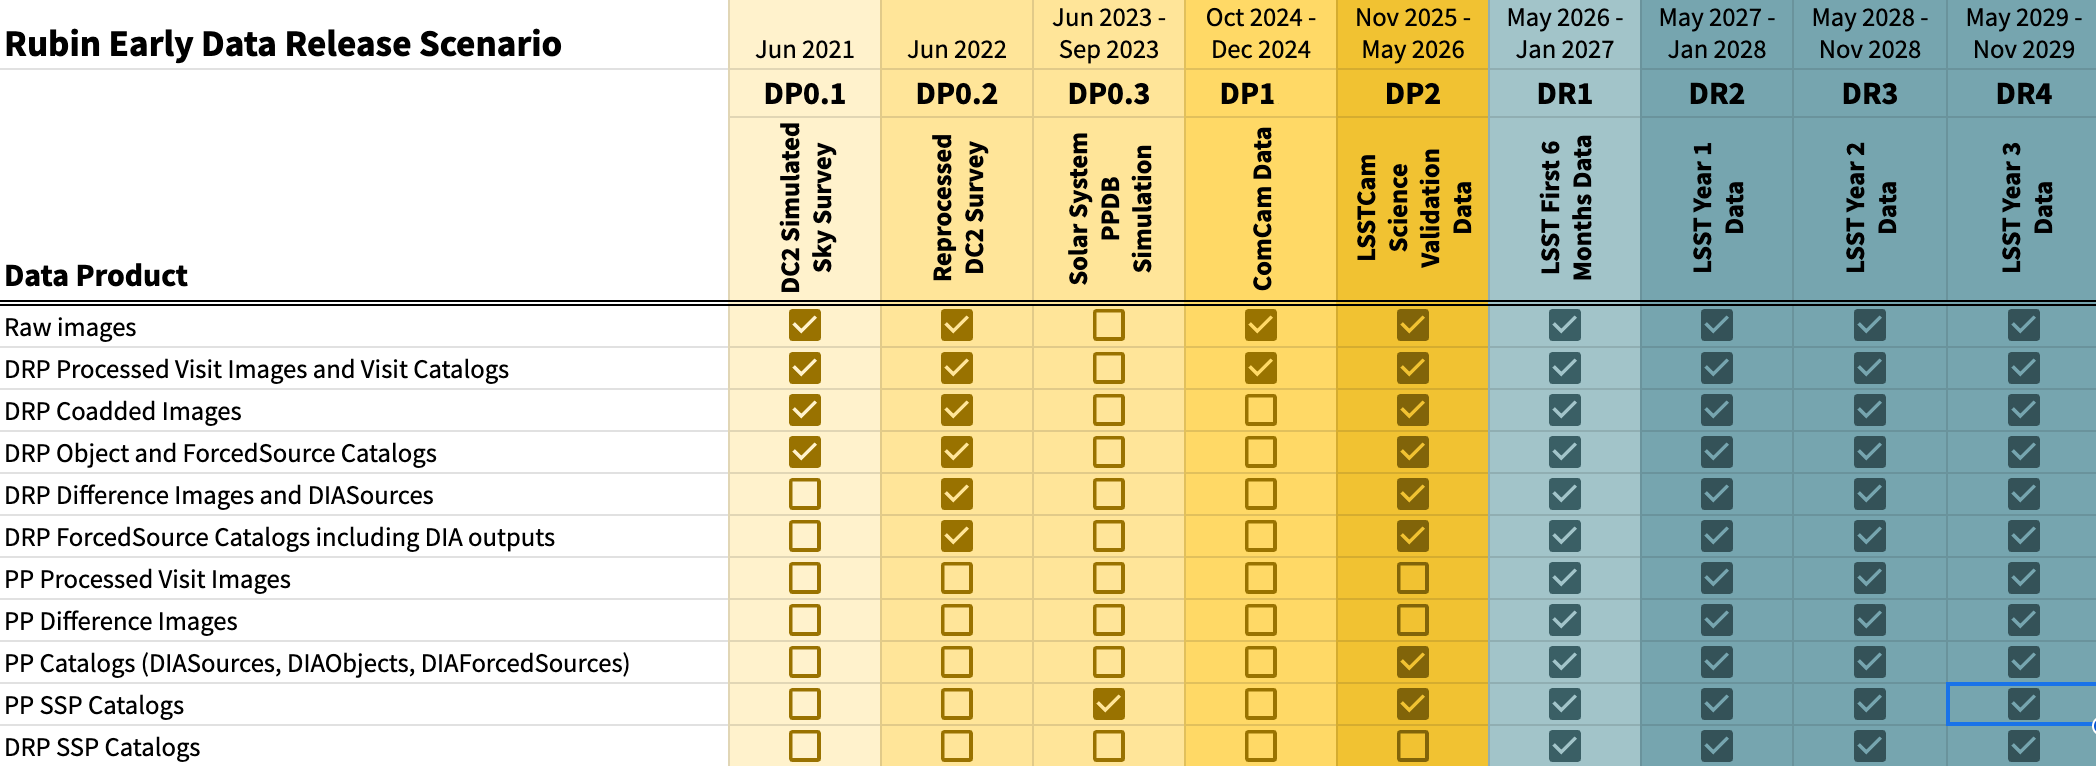
\includegraphics[width=\linewidth]{figures/DPR-summary}
\end{table}

% Data Preview 1 data products to be rediscussed following construction project replan. 
%\begin{table}
%\caption{Summary of data products expected in DP1, as of October 2022.}
%\label{tab:dp-one-products}
%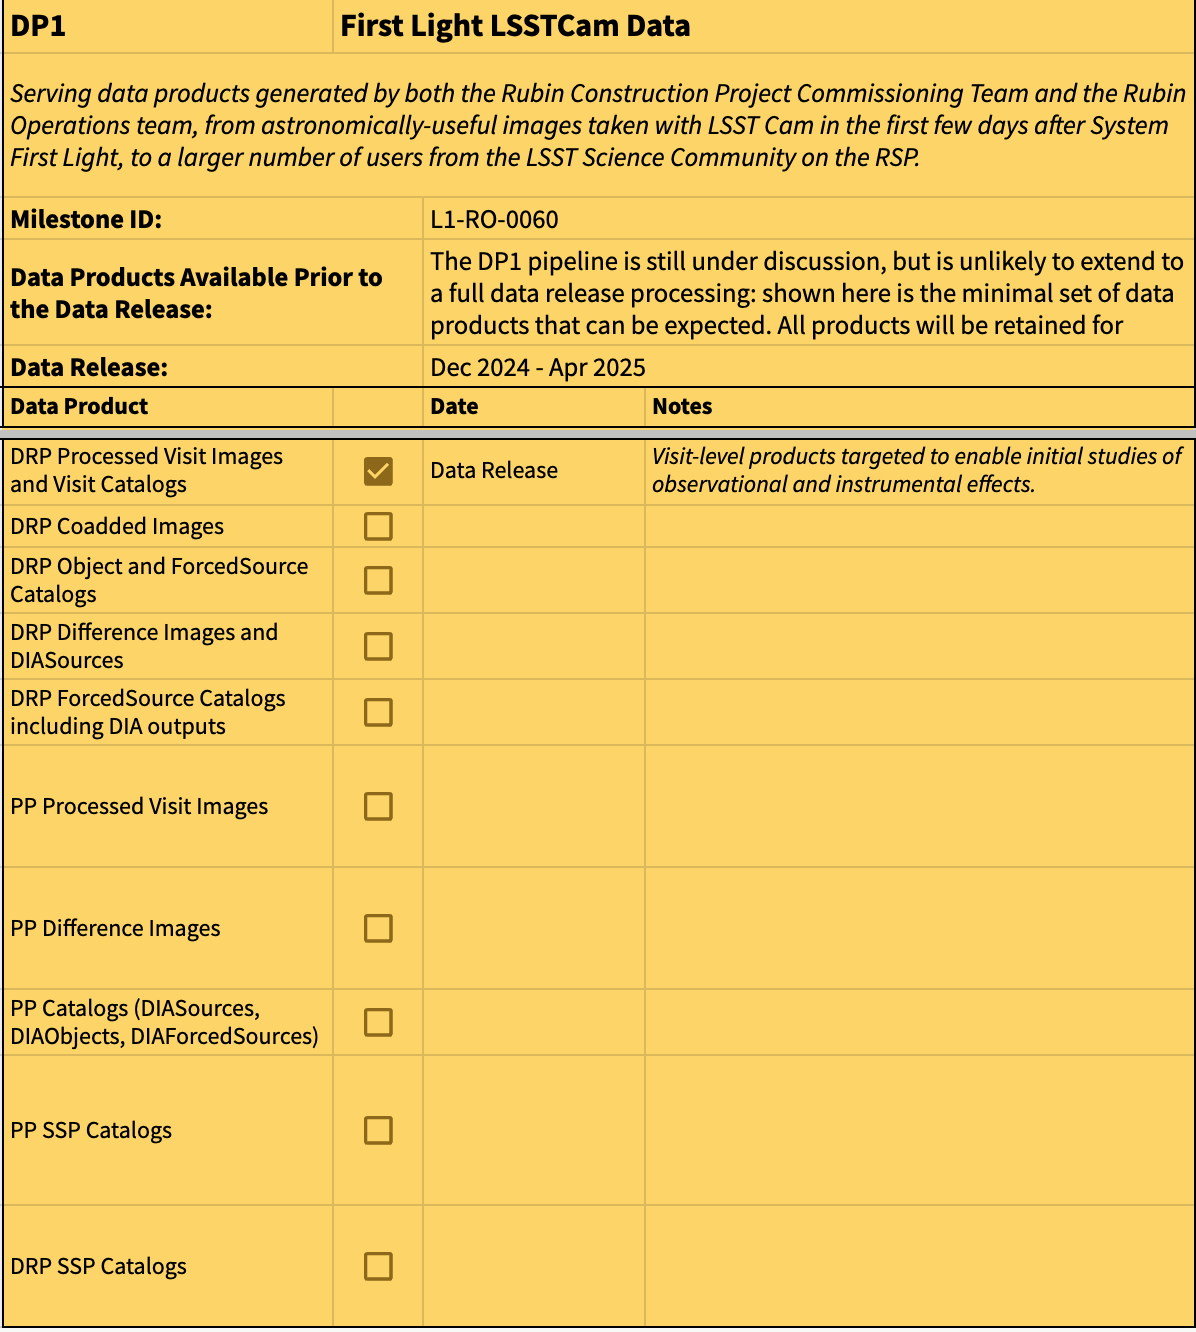
\includegraphics[width=\linewidth]{figures/DP1-products}
%\end{table}

\begin{table}
\caption{Summary of data products expected in DP2, as of October 2022.}
\label{tab:dp-two-products}
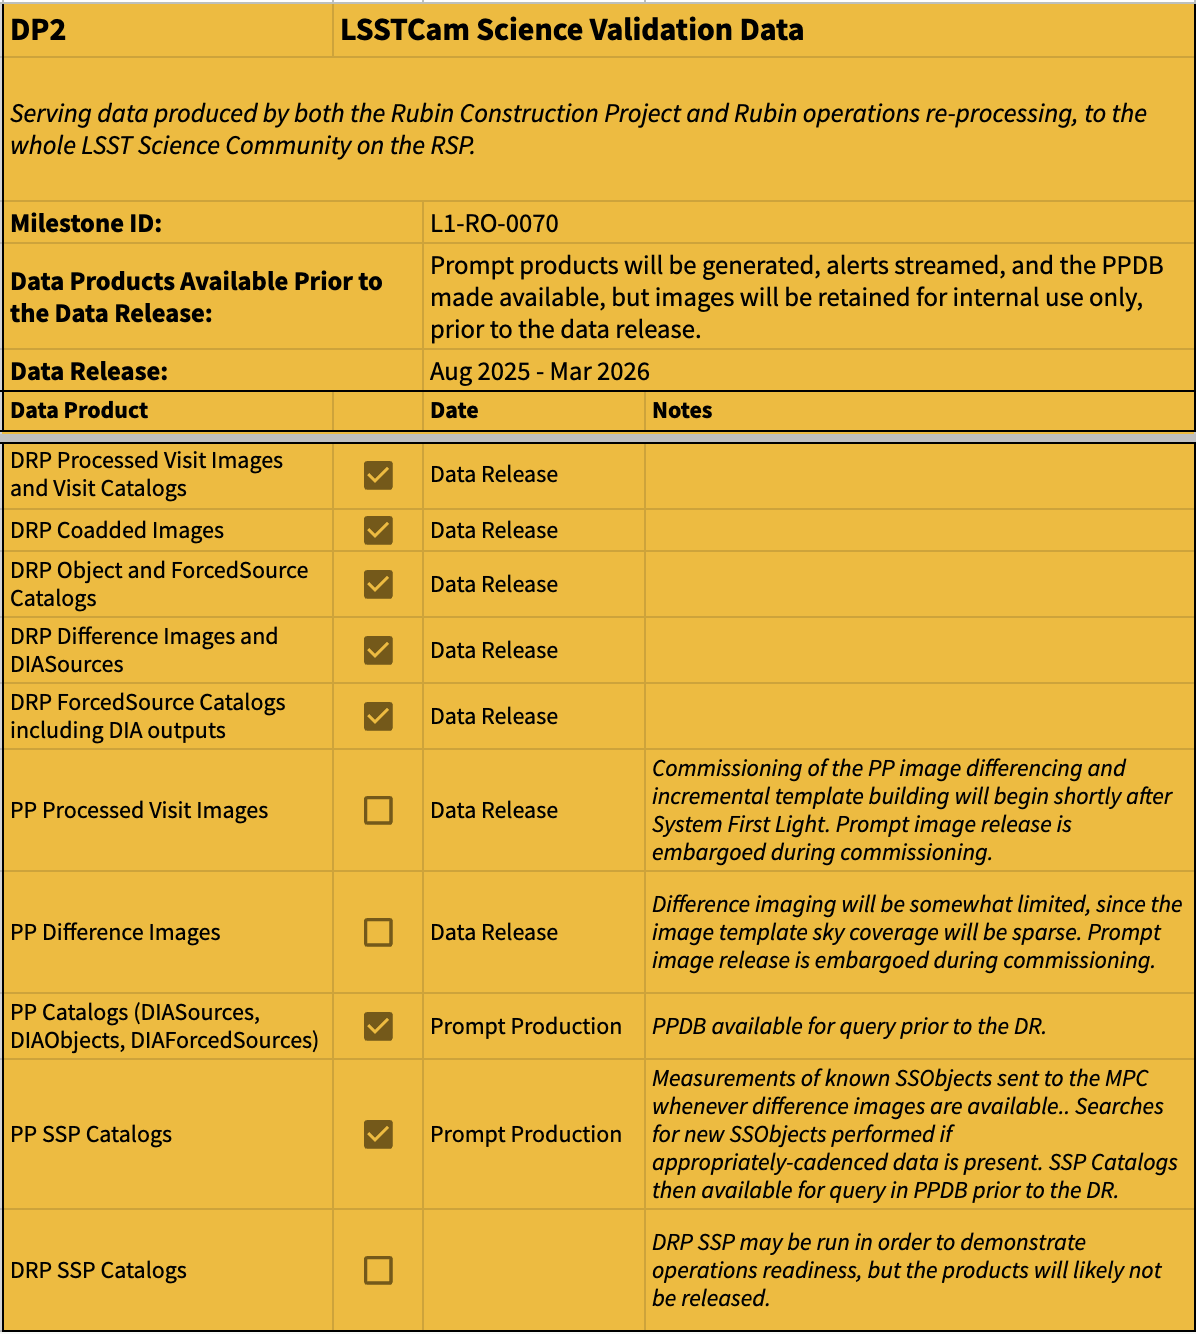
\includegraphics[width=\linewidth]{figures/DP2-products}
\end{table}

\begin{table}
\caption{Summary of data products expected in DR1, as of October 2022.}
\label{tab:dr-one-products}
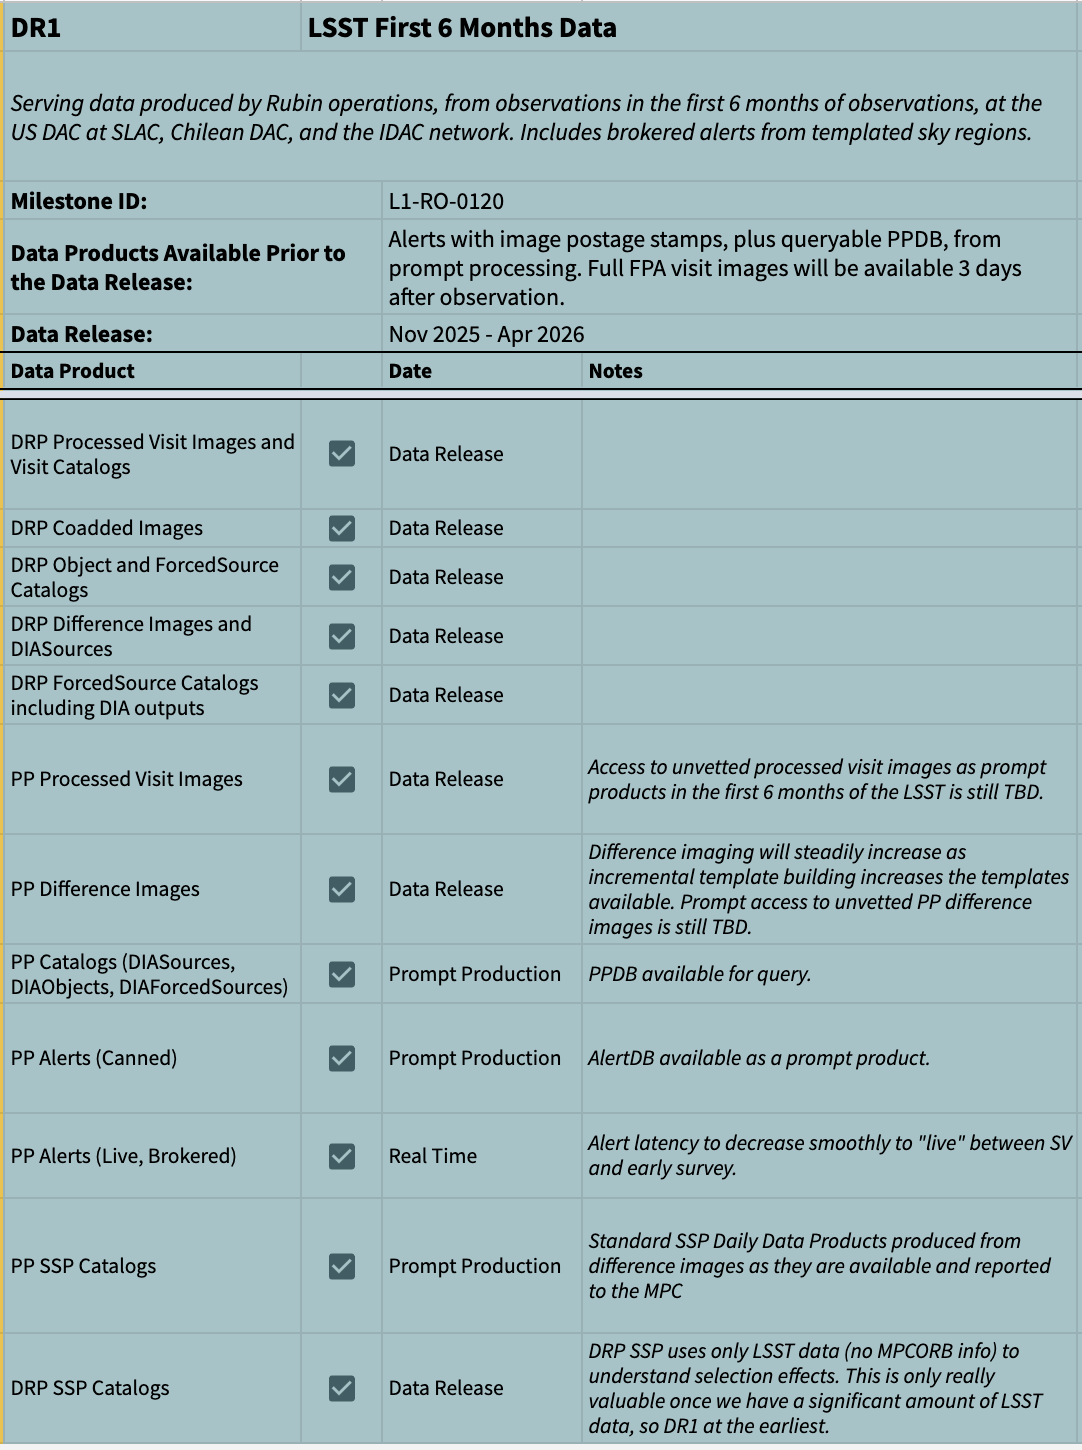
\includegraphics[width=\linewidth]{figures/DR1-products}
\end{table}


\subsection{Access to Early Science  Data Products} \label{ssec:dataaccess}
Alerts are fully world-public and will be accessible via one or more of the nine Rubin-endorsed Community Brokers\footnote{See \url{https://www.lsst.org/scientists/alert-brokers}}.
All other data products listed in \S~\ref{ssec:dataproductsummary} will be accessible to Rubin Data Rights community via the Rubin Science Platform, \citep{LSE-319}.

DP0.1 and DP0.2 are available via the RPS running at the Interim Data Facility (IDF) hosted on the Google Cloud Platform.
The IDF is considered a production environment to support Data Preview releases. 

